% !TEX TS-program = lualatex

\documentclass{tutodoc}

\usepackage{../preamble.cfg}


\begin{document}

\section{Motivations}

This project was born out of a desire to enhance \LUADRAW\ with a set of color palettes to easily produce graphics like the 3D plot shown below.
%
Despite the availability of palette generation tools such as \coolors, the choice has been made to offer pre-built palettes, because this serves several key purposes for non-designers.
%
\begin{itemize}
    \item \textbf{Reduced cognitive load:} pre-configuration eliminates design decisions, allowing to focus on content.

    \item \textbf{Consistency:} it becomes easy to ensure visual coherence across documents and projects, regardless of technology.

    \item \textbf{Accessibility compliance:} some pre-configured palettes guarantee colorblind-safe combinations.

    \item \textbf{Perceptual uniformity:} most palettes ensure distinguishable and meaningful colors for data visualization, while others serve artistic purposes.
\end{itemize}


\begin{center}
    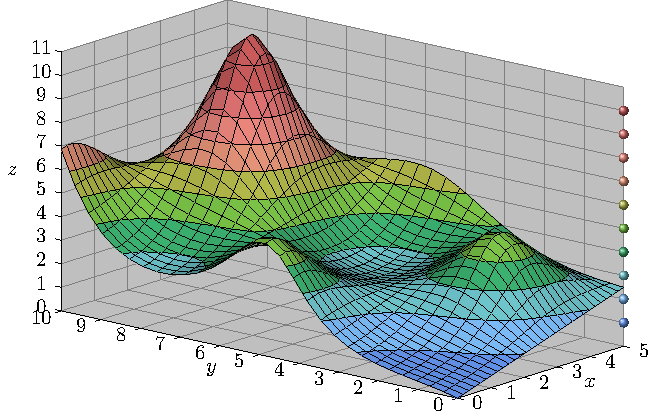
\includegraphics{../../../common/graphics/surface.pdf}
\end{center}


% -------------------- %


Technically, to generate the graphics in this section, \LUADRAW\ is provided with a finite list of colors and uses linear interpolations to calculate the intermediate color values. In the example above, the finite color palette used is defined as follows.
%
\begin{center}
    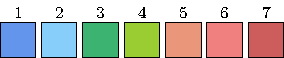
\includegraphics{../../../common/showcase/GeoRainbow-palette.pdf}
\end{center}

Using this palette, \LUADRAW\ can produce the following spectrum, allowing us to create the graphic above.
%
\begin{center}
    
\includegraphics{../../../common/showcase/GeoRainbow-spectrum.pdf}
\end{center}


% -------------------- %


\begin{tdocnote}
    Using the \lua\ implementation of \thisproj, see the section \ref{products-lua}, via \LUADRAW, we can create the palettes below made from the previous one named \tdoccodein{lua}+'GeoRainbow'+. Each instruction used is given below each palette.
    %
    \begin{center}
        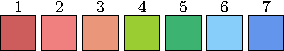
\includegraphics{../../../common/graphics/palette-reversed.pdf}

        \tdoccodein{lua}+getPal('GeoRainbow', {reverse = true})+

        \smallskip
        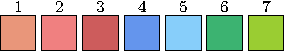
\includegraphics{../../../common/graphics/palette-shift.pdf}

        \tdoccodein{lua}+getPal('GeoRainbow', {shift = 3})+

        \smallskip
        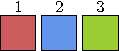
\includegraphics{../../../common/graphics/palette-extract.pdf}

        \tdoccodein{lua}+getPal('GeoRainbow', {extract = {7, 1, 4}})+
    \end{center}

    \smallskip

    This features provide remarkable creative flexibility: with the same surface as before, using the setting
    \tdoccodein{lua}+getPal('GeoRainbow', {extract = {6, 5, 4, 3, 1, 2}})+
    instead of
    \tdoccodein{lua}+getPal('GeoRainbow')+,
    we change the visual tone, shifting from a seaside feel to a snow-covered world.
    %
    \begin{center}
        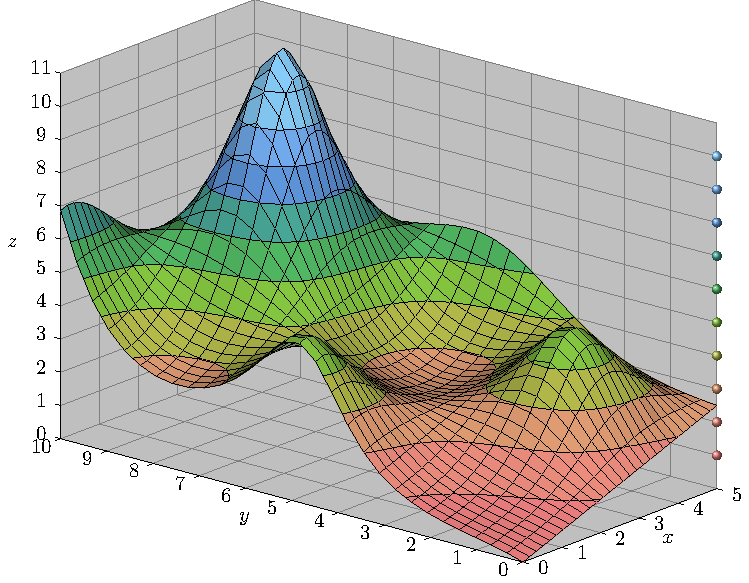
\includegraphics{../../../common/graphics/surface-options.pdf}
    \end{center}
\end{tdocnote}

\end{document}
